\documentclass[10pt,a4paper]{article}
\usepackage[utf8]{inputenc}
\usepackage[spanish]{babel}
\usepackage{amsmath}
\usepackage{amsfonts}
\usepackage{amssymb}
\usepackage{graphicx}
\usepackage{natbib}
\usepackage{lineno}
\usepackage{ragged2e}
\usepackage{multicol}
\setlength\columnsep{37pt}
\usepackage{enumerate} 
\usepackage[left=1.94cm,top=1.59cm,right=1.9cm,bottom=0.59cm]{geometry} 
\usepackage{fancyhdr}
\usepackage{url}
\usepackage{cite} 


\begin{document}
		
		\begin{center}
			\huge \textbf{Business Model Canvas aplicado a una empresa} 
		\end{center}
		\vspace{\baselineskip}
		\begin{center}
			
\includegraphics[scale=0.37]{./Imagenes/logo}
		\end{center}
		\begin{multicols}{2}
			\small
			\begin{center}
				Nelia Escalante Marón\\
				2014049551\\
				UPT - Ingenierí­a de Sistemas\\
				EPIS\\
				Tacna, Perú\\
				\vspace{\baselineskip}
				Yerson Coaquira Calizaya\\
				2015053225\\
				UPT - Ingenierí­a de Sistemas\\  
				EPIS\\
				Tacna, Perú\\                 
				\vspace{\baselineskip}
				Flor Condori Gutierrez\\
				2015053227\\
				UPT - Ingenierí­a de Sistemas\\ 
				EPIS\\	
				Tacna, Perú\\                 
				\columnbreak
				
				\vspace{\baselineskip}
				Christian Cespedes Medina\\
				2010036256\\
				UUPT - Ingenierí­a de Sistemas\\  
				EPIS\\	
				Tacna, Perú\\                

				\vspace{\baselineskip}
				Javier Octavio Arteaga Ramos \\
				2007028981\\
				UPT - Ingenierí­a de Sistemas\\  
				EPIS\\	
				Tacna, Perú\\                 

			\end{center}
			\normalsize			
		\end{multicols}
		\vspace{\baselineskip}
		\begin{multicols}{2}
		\textbf{\textit{\large Abstract}}\rule[1.5mm]{5mm}{0.1mm} El modelo Canvas cuenta con 9 bloques los cuales hacen referencia a las características de la empresa que se quiere crear. Debemos tener en cuenta que al inicio puede costarnos un poco insertar los datos necesarios en cada bloque, y eso puede deberse a que el modelo de negocio aun no está bien definido.
		
		Los 9 bloques que va a llenar segun este modelo son: Propuesta de Valor, Los canales, Relaciones con los Clientes, Fuentes de ingresos, Recurso clave, Activida des principales, Alianza Clave y Estructura de Precio.
				
		\textit{The Canvas model has 9 blocks which refer to the characteristics of the company you want to create. We must take into account that at the beginning it can cost us a bit to insert the necessary data in each block, and that may be because the business model is not yet well defined.}
		
		\textit{In this final work we will apply the blocks of the BMC model to a company, these are: value proposition, channels, customer relations, revenue sources, key resource, core activities, key alliance and price structure}
		
		\vspace{\baselineskip}
			
		\textbf{\textit{\large Keybwords}}\rule[1.5mm]{5mm}{0.1mm} BMC, Web 2.0, aplicacion del Modelo Canvas a una empresa, cloud
		
		\columnbreak
		
		\section{Marco Teórico} 
		
		Todo emprendedor posee una idea de negocio, sin embargo, su puesta en práctica no resulta fácil, y mucho menos sacarle rentabilidad. Por ello contamos con varias estrategias, entre ellas el modelo Canvas. Estas estrategias buscan asegurarnos de que nuestras iniciativas llegaran a tener a éxito. Sin embargo, no todos los modelos de negocio nos dan soluciones perfectas. Es por ello por lo que surge el modelo Canvas.\\
		
		Modelo que se ha convertido desde el 2008 como herramienta estrella en la gestión estratégica y empresarial de un negocio. El modelo Canvas permite ver y moldear en un solo folio, estructurado en nueve elementos, cual es el modelo de nuestro negocio.  Y lo mejor de todo, es tan sencillo que puede ser aplicado en cualquier escenario, ya sea una pequeña, mediana y gran empresa.  Además, no sólo sirve para las nuevas empresas sino también para aquellas que ya están establecidas. \\
		
		En definitiva, este modelo trata de aprender muy rápido sobre el mercado, en un corto tiempo y con el mínimo coste.  Con el objetivo de lograr un modelo que busque la agilidad y la reducción del tiempo en el desarrollo de iniciativas empresariales, para finalmente generar productos y servicios que cumplan con las necesidades de los clientes y aporten valor.\\
		
		\textbf{¿En qué consiste el modelo Canvas?}\\
		
		En la descripción de un modelo de negocio dividido en nueve módulos básicos que reflejen el método para obtener ingresos en una empresa.  
		
		\begin{enumerate}[1.]
			\item \textit{Segmentos de clientes}
			
			La empresa debe definir en el bloque de segmentos de clientes cuál es el nicho de mercado que pretende alcanzar. Con el fin de satisfacer mejor a los clientes, una empresa puede agruparlos en distintos segmentos con necesidades, comportamientos u otros atributos comunes. Un modelo de negocio puede definir uno o varios segmentos a los cuales va a servir (al mismo tiempo está descartando otros nichos de clientes).\\
						
			Sin el nicho o segmento de clientes no es rentable, la empresa no puede sobrevivir por mucho tiempo. Por ello el segmento se define si las necesidades requieren y justifican una producto o servicio distinto, si es posible llegar a ellos a través de canales de distribución diferentes, están dispuestos a pagar el precio por el valor que obtienen y si se obtienen beneficios sustanciales.\\
			
			El modelo Canvas establece que hay varios tipos de segmentos de clientes, tales como mercado masivo (donde el modelo de negocio no se distingue entre uno y otro, se centra en un grupo grande de clientes con necesidades más o menos similares), nicho de mercado (se centra en un segmento especifico de clientes especializados y sus necesidades particulares), segmentado (clientes del mismo nicho con necesidades ligeramente diferentes), diversificado (cuenta con varios nichos o segmentos de clientes).
			
			\item \textit{Propuestas de Valor}
			
			En este bloque se describe el paquete de productos y servicios que crean valor para un segmento especifico de clientes.\\
			
			El modelo define que una propuesta de valor es la razón por la que los clientes recurren a una empresa en lugar de otra para resolver su problema o necesidad. Es el conjunto o paquete de beneficios que una empresa ofrece a sus clientes. Implica responder a preguntas como: ¿Qué valor damos a los clientes?, ¿Cuál de los problemas de nuestros clientes estamos ayudando a resolver?, ¿Qué necesidades de los clientes estamos satisfaciendo?, ¿Cuáles paquetes de productos y servicios ofrecemos para cada segmento de clientes?\\
			
			Las propuestas de valor pueden ser:
			
			\begin{itemize}
				\item Innovadoras: Mejoran el producto, el proceso o sus beneficios en función de las necesidades del cliente.
				\item Funcionales: Pueden ser similares a otras existentes en el mercado, pero con más funciones y atributos.
				\item Novedosas: Al satisfacer un conjunto totalmente nuevo de necesidades que antes no eran percibidas.
				\item De alto rendimiento: Mejora el rendimiento del producto o servicio.
				\item Personalizada: Adaptación de productos y servicios a necesidades específicas de sus clientes.
				\item De diseño: Un producto puede destacar por un diseño superior.
				\item De marca: Los clientes encuentran valor en el simple hecho de utilizar y visualizar una marca específica.
				\item Precio: Reciben un valor similar a un precio inferior y ayuda a los clientes a reducir sus costos
				\item Accesible: Lograr que los clientes tengan acceso a productos y servicios que anteriormente no podían disponer
				\item Conveniencia y usabilidad: Hacer que los productos sean más fáciles de usar y que resuelvan una necesidad oportuna.
			\end{itemize}
			
			\item \textit{Canales}	
			
			En este bloque la empresa establece cómo se va a llevar los productos o servicios hasta sus clientes indicando los mecanismos de distribución, contacto, venta, soporte y mantenimiento.\\
						
			Los canales -dicen los creadores del modelo de negocios Canvas- cumplen varias funciones: sensibilizan a los clientes, ayudan a los clientes a evaluar la propuesta de valor de la empresa, permite que los clientes compren productos y servicios específicos, entregan la propuesta de valor a los clientes, y proporcionan atención posterior a la compra.\\
			
			Aquí, se debe responder a preguntas: ¿Cómo quiere llegar hasta los clientes?, ¿Cómo son nuestros canales integrados?, ¿Cuáles funcionan mejor?, ¿Cuáles son los más costosos y eficientes?, ¿Cómo las vamos a integrar a las rutinas del cliente?\\
			
			El modelo Canvas establece varias clases de canales: propios, directos, indirectos y asociados. Una empresa debe encontrar la combinación adecuada para satisfacer a los clientes. Para definir esta mezcla debe calcular cuáles son los costos de cada uno y cuáles le aportan más utilidades.
			
			\item \textit{Relaciones con el Cliente}
			
			Una empresa debe tener claro el tipo de relación que quiere establecer con cada segmento de clientes: adquisición de clientes, retención de clientes o impulsar las ventas (upselling).\\
			
			Al inicio se pueden establecer estrategias agresivas de adquisición de clientes; luego se pasa a estrategias para retener la clientela actual; y después para lograr que los clientes compren más.\\
			
			Para eso es necesario tener servicios de asistencia personal (la relación se basa en la interacción humana a través de un ejecutivo específico), autoservicio o servicios automatizados, redes sociales (para crear comunidades de clientes que permiten a los usuarios intercambiar conocimientos y solución de problemas), y co-creación (donde el cliente sugiere, critica, califica y comenta).
			
			\item \textit{Fuentes de Ingresos}
			
			El bloque de ingresos debe responder a la pregunta sobre cuáles son los valores por los cuales los clientes estarán dispuestos a pagar y cuáles son las fuentes de ingresos para cada segmento de clientes, que pueden ser: 
			
				\begin{itemize}
					\item Pagos directos de los clientes, de una sola vez.
					\item Los ingresos derivados de pagos escalonados o segregados por mes.
					\item Venta de derechos de propiedad sobre un producto físico.
					\item Cuotas de suscripción o mensualidades.
					\item Prestamos, renting o alquiler forma sobre la concesión del derecho exclusivo a utilizar un activo.
					\item Licencias o permiso para usar productos o servicios protegidos por la propiedad intelectual.
					\item Corretajes: deriva de la intermediación de servicios prestados.
					\item Publicidad: ingresos derivados de tarifas de publicidad de un determinado producto, servicio o marca
				\end{itemize}
			Cada flujo de ingresos puede tener precios diferentes o utilizar modalidades de precios fijos o precios dinámicos.\\
			
			Aquí, se debe responder a preguntas como: ¿Cuál propuesta de valor están nuestros clientes realmente dispuestos a pagar?, ¿Cómo prefieren pagar?, ¿Cuánto contribuyen a los ingresos totales?
			
			\item \textit{Recursos clave}
			
			Este bloque enumera los recursos y activos que se requieren para implementar el modelo de negocio, para crear una propuesta de valor, establecer los canales, mantener relaciones con los segmentos de clientes y obtener ingresos.\\
			
			Evidentemente se requieren diferentes recursos (físicos, financiero, intelectuales o humanos) para cada tipo de modelo de negocio. Además, se indica si cada recurso es de propiedad de la empresa o si es arrendado.	
				\begin{itemize}
					\item \textit{Recursos físicos:} Instalaciones de manufactura, edificios de oficinas, vehículos, máquinas, sistemas de punto de venta, redes distribución, logística e infraestructura.
					\item \textit{Recursos intelectuales:} Marcas, patentes, derechos de autor y bases de datos.
					\item \textit{Recursos humanos:} Tipo de recursos que se requieren
					\item \textit{ Recurso financiero:} Necesidad de dinero en efectivo, líneas de crédito, arrendamiento, socios inversionistas, salida a bolsa de valores o una agrupación de opciones.
				\end{itemize}
			
			\item \textit{Actividades Principales}
			
			En este bloque se incluyen las actividades más importantes que una empresa debe realizar para implementar el modelo de negocio. Cada modelo requiere una serie de actividades claves distintas.\\
			
			Dependiendo del tipo de negocio, las actividades incluyen el diseño, el desarrollo, la gestión de la cadena de suministro, la fabricación, los servicios, desarrollo y sostenimiento de la plataforma y del sistema de pagos, la gestión del conocimiento y formación continua, y la entrega de un producto de alta calidad.[\citen{practice}]
			
			\item \textit{Alianzas}
			
			El bloque de asociaciones o alianzas establece la red de proveedores y socios que se requieren para implementar exitosamente y optimizar el modelo de negocio, reducir los riesgos, lograr economías de escala o adquirir recursos.\\
			
			Se distinguen entre cuatro tipos de asociaciones diferentes: alianzas estratégicas entre no competidores, alianzas estratégicas entre competidores, empresas conjuntas para el desarrollo de nuevos negocios, y para adquisición de activos e insumos.\\
			
			Las alianzas permiten ampliar sus propias capacidades, apoyarse en otras empresas para proporcionar recursos particulares o realizar ciertas actividades, adquirir conocimientos o licencias, o acceder a los clientes.\\
			
			En este caso se responde a preguntas claves como: ¿Quiénes son nuestros socios principales?, ¿Quiénes son nuestros principales proveedores?, ¿Que recursos claves estamos adquiriendo de los socios?, ¿Qué actividades clave realizan los socios?
			
			\item \textit{Estructura de Datos}
			
			La estructura de costos describe todos los costos incurridos para operar un modelo de negocio, la creación y entrega de valor, el mantenimiento de relaciones con los clientes y la generación de todos los ingresos.\\
			
			Tales costos se pueden calcular con relativa facilidad después de definir los recursos claves, las actividades clave y las principales alianzas y deben responder a preguntas como: ¿Cuáles son los costos más importantes inherentes a nuestro negocio modelo?, ¿Cuáles son los recursos y las actividades clave de mayor costo?\\
El modelo de Canvas indica que “como es natural”, los costos deben reducirse al mínimo en cada modelo de negocio, aunque las estructuras de más bajo coste son más importante para algunos modelos de negocio que para otros.\\
			
			En este caso se distingue entre dos estructuras: uno centrado en minimizar los costos, donde el primero se preocupa por reducir al máximo los costos para tener un precio y beneficios adecuados; y otro basado en la propuesta de valor, donde no hay tanta preocupación por el costo y el precio, pero si por la creación de un valor premium con proposiciones y un alto grado de servicio personalizado.\\
			
			La estructura de costos incluye aquellos que son fijos (no varían, aunque se aumente la producción, tales como salarios, alquileres, e instalaciones) y variables (varían proporcionalmente con el volumen de bienes o servicios producidos como materia prima y otros insumos).\\
			
			Las empresas pueden intentar lograr economías de escala mediante la reducción de costos de insumos al comprar en mayor volumen, donde el costo promedio por unidad cae a medida que aumenta la producción o economías de alcance, donde se crean ventajas al incrementar el alcance de las operaciones.[\citenum{ de2013valencia}	]			
		\end{enumerate}
		
		\textbf{Estructura del modelo Canvas}		
		\begin{center}
			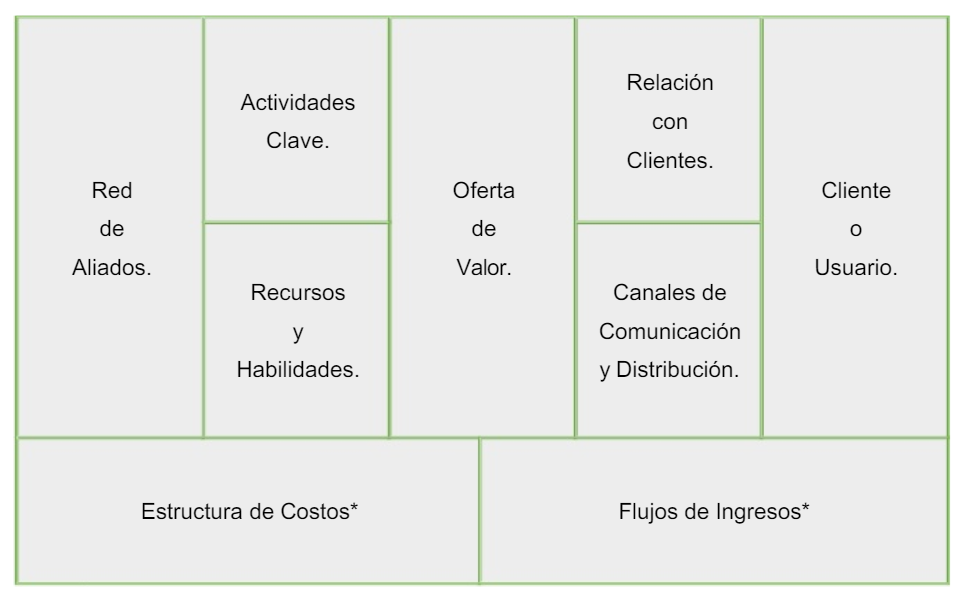
\includegraphics[scale=0.30]{./Imagenes/img01}
		\end{center}
		
		\textbf{Ventajas y Desventajas del BMC}
		
		\begin{enumerate}[A.]
			\item Ventajas
				\begin{itemize}
					\item Simplicidad de interpretación. La distribución organizada de los 9 elementos permite dicha simplicidad. 
					\item Enfoque integral y sistémico. La interpretación de todos los elementos hace más visible cualquier posible incoherencia. 
					\item Cambios y repercusiones. El análisis de cada alternativa nos permite tantear la viabilidad de cambios
					\item Cualquier tamaño, cualquier actividad. Es un modelo aplicable a todo tipo de negocio, con independencia de su objeto y de su cifra de negocio
					\item Sinergia y trabajo en equipo. La simplicidad del método facilita la generación de ideas y distintos aportes de un grupo de personas que se reúna para desarrollarlo. 
					\item Análisis estratégico en una hoja. Poderosa herramienta para el análisis estratégico: FODA, análisis del mercado, competidores, clientes, proveedores, estructuras y procesos. 
				\end{itemize}
			
			\item Desventajas
				\begin{itemize}
					\item Poco precisa, no sirve para operativa concreta
					\item Se debe complementar con mapa de procesos detallados
					\item Por ser tan novedosa puede hacernos creer que completando el lienzo ya tenemos el modelo resuelto
				\end{itemize}
		\end{enumerate}	
		
		\section{Desarrollo}
		
		Vamos a estar revisando o creando el modelo de negocio de la empresa UBER. 		
		Lo primero que hacemos es generar nuestro Canvas con cada uno de los nueve bloques.\\
					
		\textbf{Estructura del modelo Canvas}		
		\begin{center}
			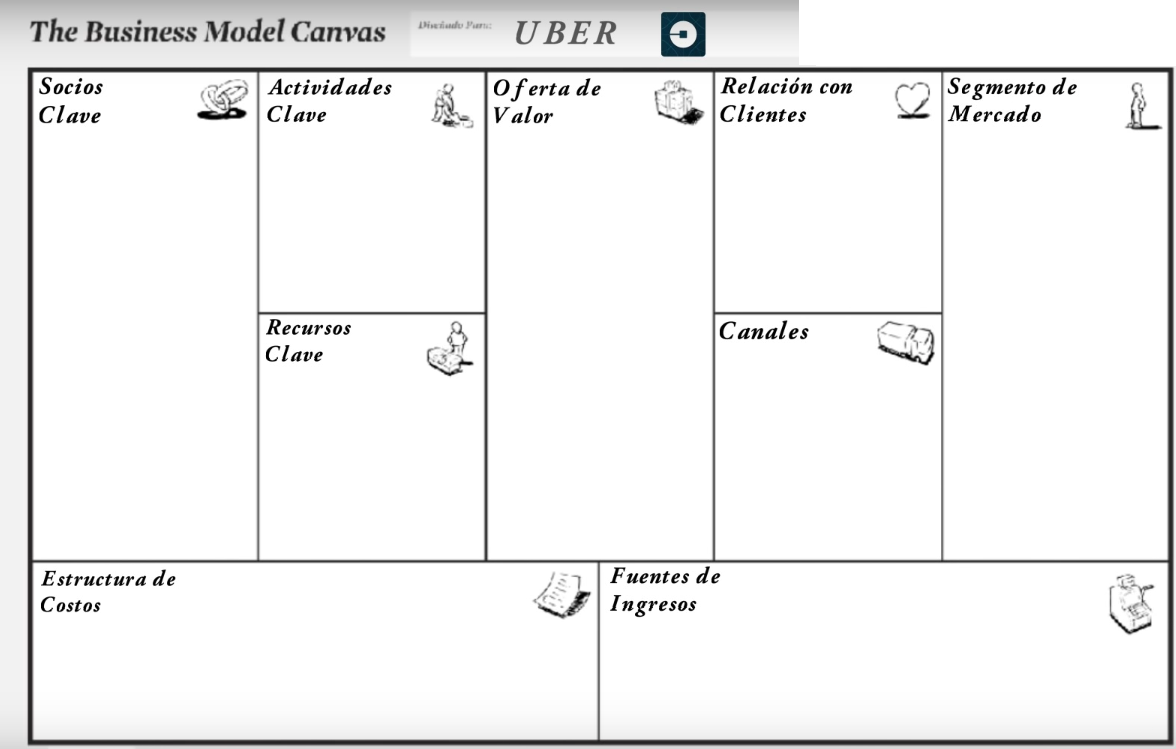
\includegraphics[scale=0.30]{./Imagenes/img02}
		\end{center}
		
		Una vez que tenemos la vista general de nuestro canvas lo escribimos la descripción información de quien está realizando importantes poner la fecha y la iteración con la que estamos trabajando eso nos permitirá constantemente seguir avanzando con el iniciamos con el bloque.
				
		\begin{enumerate}[a.]
			\item OFERTA DE VALOR 
			
			Para este segmento de mercado tenemos que identificar claramente cuál es su oferta de valor.\\
			
			Oferta de valor para usuarios:
			
				\begin{itemize}
					\item Los tiempos reducidos de respuesta 
					\item Se cobra el servicio por kilómetros recorridos siempre teniendo la visibilidad de la información del precio de la tarifa que nos van a cobrar.
					\item Información del conductor.
					\item Visibilidad de la ruta con la que estamos transportando nos eso nos da una seguridad en el servicio que estamos tomando. 					
				\end{itemize}
				
				\begin{center}
					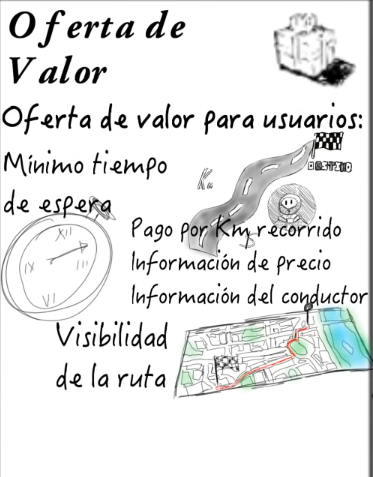
\includegraphics[scale=0.30]{./Imagenes/img03}
				\end{center}
			
			Oferta de valor para conductores :

				\begin{itemize}
					\item Fuente de ingresos extra a la que normalmente cuenta la persona y como también lo decíamos pues puede ser la principal fuente de ingresos. 
					\item Flexibilidad tanto en días de trabajo como en horarios.
					\item Facilidad de pago para recibir sus ingresos  
				\end{itemize}
				
				\begin{center}
					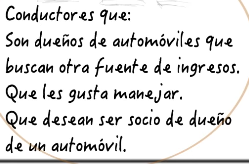
\includegraphics[scale=0.55]{./Imagenes/img04}
				\end{center}
			
			\item SEGMENTOS DE MERCADO 
			
			En el cual identificamos quiénes son los principales actores que debemos de conocer el primero son los usuarios que usan la plataforma de uber los cuales los podemos clasificar de la siguiente forma.\\
			
			Usuario que:
			\begin{itemize}
				\item Son personas que no cuentan con automóvil
				\item No quieren conducir por diversa razones
				\item Buscan viajar con estilo VIP(comodamente)
				\item Buscan servicio de calidad
			\end{itemize}
		
			\begin{center}
				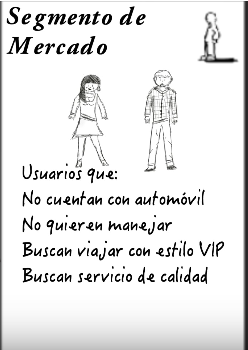
\includegraphics[scale=0.55]{./Imagenes/img05}
			\end{center}
				
			Los conductores del servicio de uber eso los podemos clasificar de la
			siguiente forma:
			\begin{itemize}
				\item Son dueños de automóviles que buscan otra fuente de ingresos bueno en algunos casos como la principal fuente de ingresos. 
				\item Que les gusta manejar 
				\item que desean ser socios de dueños de automóvil en el caso de no contar con uno propio
			\end{itemize}
		
			\begin{center}
				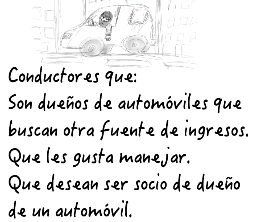
\includegraphics[scale=0.55]{./Imagenes/img06}
			\end{center}
			
			\item RELACIÓN CON CLIENTES
			
			En la parte de relación con clientes dado que es una plataforma este que se maneja en internet social media es es la principal relación que tienen con los clientes otra de las formas que tiene para relacionarse con los clientes es por medio de las reseñas y las calificaciones que se le da a los conductores y por último ofrece una parte una plataforma de soporte técnico tanto para los usuarios como para los conductores.
			
			\begin{center}
				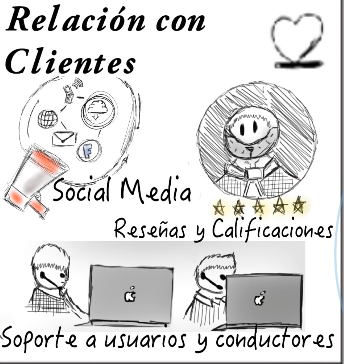
\includegraphics[scale=0.55]{./Imagenes/img07}
			\end{center}
		
			\item CANALES
			
			Con los que hubiera se llegar su oferta de valor y sus segmentos de mercado la principal dado que la plataforma sí lo es son las aplicaciones móviles tanto en las versiones de android Windows phone y iOS de Apple y por último los sitios web tanto el personal y de terceros.
			
			\begin{center}
				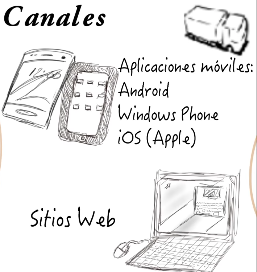
\includegraphics[scale=0.55]{./Imagenes/img08}
			\end{center}
			
			\item ACTIVIDADES CLAVE 
			
			En donde la principal actividad es el desarrollo de la plataforma tanto de las aplicaciones como los sistemas de soporte y administración por otro lado otra actividad clave es la evaluación de lo que son los conductores y toda la parte de administración de contratos con ellos y por último por las actividades de marketing y ventas que requieren para colocar la marca después.
			
			\begin{center}
				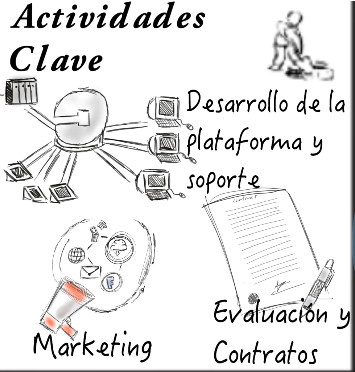
\includegraphics[scale=0.55]{./Imagenes/img09}
			\end{center}
		
			\item RECURSOS CLAVE
			Los principales recursos clave con los que se requiere über para operar es:
			
			\begin{itemize}
				\item Plataforma tecnológica toda la infraestructura de plataforma tecnológica.
				\item Conductores expertos verificados.
			\end{itemize}
			
			 \begin{center}
			 	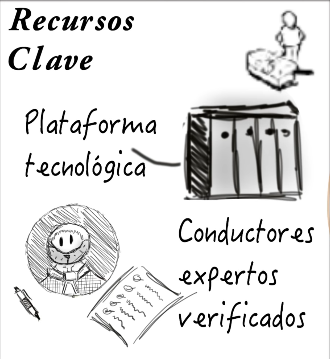
\includegraphics[scale=0.55]{./Imagenes/img10}
			 \end{center}
		 
			\item SOCIOS CLAVE 	
			
			Son:
			
			\begin{itemize}
				\item Los conductores que son encontrados tanto como socio clave dado que ellos son los que cuentan con los automóviles y los skills pero también son clientes porque requerimos mantenerlos contentos.
				\item Proveedores de los mapas UBER no tiene mapas propios por lo tanto requiere esa esa característica buscarla en un tercero. 
				\item Los inversionistas esos permiten la viabilidad económica del negocio
			\end{itemize}
		
			 \begin{center}
				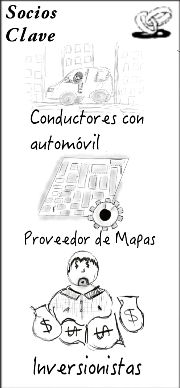
\includegraphics[scale=0.55]{./Imagenes/img11}
			\end{center}
			
			\item ESTRUCTURA DE COSTOS 
			
			Donde descubrimos que los principales costos son la:
			
			\begin{itemize}
				\item Infraestructura tecnológica 
				\item Grupo de colaboradores que tiene de planta para operarla el negocio  
				\item Actividades de marketing ventas para lo que es la colocación de la marca principalmente.
			\end{itemize}
		
		 	\begin{center}
				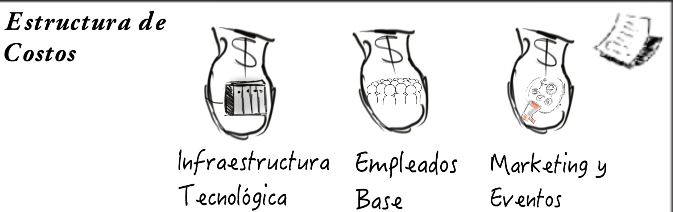
\includegraphics[scale=0.45]{./Imagenes/img12}
			\end{center}
		
			\item FUENTES DE INGRESO  
			
			Que básicamente es todo lo que le estamos vendiendo a nuestros nuestros clientes y bueno en el caso de uber es una plataforma de servicio de transporte privado y se cobra por medio de una tarifa de kilómetro recorrido la cual es calculada con respecto a la demanda que se tenga en el momento y también cuenta con una serie de servicios como por ejemplo über taxi tradicional, uber black con mejores vehículos, über x ,Uber Pool, Uber SUB, Uber Cargo.\\
			
			Con esto vemos curva ya con el canvas vemos una vista completa de lo que es todo el negocio desde aquí podemos saber exactamente cómo es cómo opera también nos permite generar nuevas hipótesis las cuales podríamos probar haciéndole las modificaciones a nuestros canvas o podríamos modelar un nuevo negocio.
			
			\begin{center}
				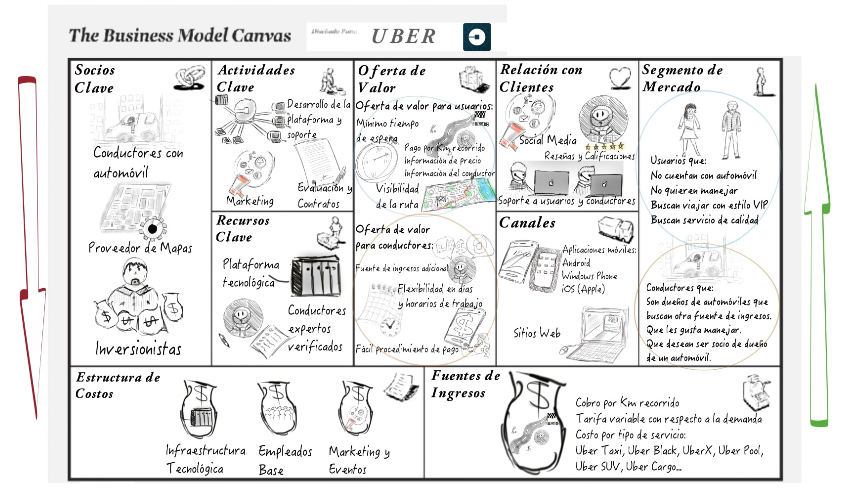
\includegraphics[scale=0.38]{./Imagenes/img13}
			\end{center}
						
		\end{enumerate}
		
		\bibliographystyle{apalike}
		\bibliography{BIBLIO}		
	
		\end{multicols}	
			
\end{document}}